\documentclass[11pt, twoside, reqno]{book}
\usepackage{amssymb, amsthm, amsmath, amsfonts}
\usepackage{graphicx}
\usepackage{color}
\usepackage{hyperref}
\usepackage{verbatim}
\usepackage[toc,page]{appendix}
\usepackage{listings}
\appendixpageoff

\usepackage{bardtex}

%The following optional command allows for a change in the method of inputting the bibliography.  The options are amsrefs'' and bibtex."  If the command is not used, the default is amsrefs.''  The bibliographic entries given at the end of this file are in the amsrefs format; a different format is needed for bibtex.  See the manual for details about the bibliography.

\styleoption{matproject}

%Your macros, if you have any.
\usepackage{color}
 
\definecolor{codegreen}{rgb}{0,0.6,0}
\definecolor{codegray}{rgb}{0.5,0.5,0.5}
\definecolor{codepurple}{rgb}{0.58,0,0.82}
\definecolor{backcolour}{rgb}{0.95,0.95,0.92}
 
\lstdefinestyle{mystyle}{
    backgroundcolor=\color{backcolour},   
    commentstyle=\color{codegreen},
    keywordstyle=\color{magenta},
    numberstyle=\tiny\color{codegray},
    stringstyle=\color{codepurple},
    basicstyle=\footnotesize,
    breakatwhitespace=false,         
    breaklines=true,                 
    captionpos=b,                    
    keepspaces=true,                 
    numbers=left,                    
    numbersep=5pt,                  
    showspaces=false,                
    showstringspaces=false,
    showtabs=false,                  
    tabsize=2
}
 
\lstset{style=mystyle}


\begin{document}

\titlepgmat{Predicting How People Vote From How They Tweet}{Rao Vinnakota}
    {May}{2019}

\abstr

The project observes tweets concerning the midterm elections and uses the sentiment drawn from those tweets to predict voting trends.

\tableofcontents

%\dedic

%Text of dedication.

%\acknowl

%Text of acknowledgments.

\startmain

\intro
\hspace{0.1in}Donald Trump stunned the world when he was elected President of the United States. Trump ran an unorthodox campaign, specifically in regards to his use of social media. Trump used accounts on Twitter and Facebook as a voice to attack candidates, disseminate campaign information, and engage with voters. 

Public polling in 2016 didn’t predict the upset. In fact, it didn’t come particularly close. The latest tracking polls before election day showed Clinton in the lead with a margin of anywhere from +1 to +6. Most pollsters believed that Trump would sweep strictly conservative areas, but Clinton would every state that really mattered. Obviously, that didn’t happen

If you look through tweets following the election, Trump supporters claimed that victory was inevitable, and that Trump’s social media interaction demonstrated it. true? Was Trump’s potential victory present on social media for people to see? 

That is idea my senior project explore. Can you mathematically evaluate opinions on social media to predict voting trends. I will gather tweets pertaining to the 2018 midterm elections and use the sentiment expressed in those tweets and attempt to predict voting results. 


\section{Political Polling - A Short Overview}
\hspace{0.1in} The earliest iteration of polling was a straw poll conducted in Harrisburg, Pennsylvania which showed Andrew Jackson leading John Quincy Adams in the 1824 Presidential Election. Journalists from The \textit{Harrisburg Pennsylvanian} asked local voters which they preferred. Jackson winning both the polls and the election created legitimized the poll. Polls continued to be local until the early 20th century when Literary Digest sent out postcards to reader asking for their pick of the presidential election. The Literary Digest correctly predicted 5 straight elections and opinion polls reached the national stage. 

In the advertising boom of post-World War II, most polling shifted to telecommunications. With telephones, there was an ability to reach a wider audience, ask deeper questions. Pollsters could now build a profile of a voter, and forecast more accurate results. Accompanying the advance in polling was a focus on sampling. Pollsters couldn’t call every single house in the United States. Instead, groups of people or “samples” that would accurately represent the country were called. Responses from the sample were extrapolated to cover the whole. 

Today, the digital age and social media have made polling’s barrier of entry low. A short scroll through Twitter will show hundreds of “opinion polls”. Youtube videos’ likes and dislikes function as an informal poll. The Algorithm will often promote videos that are more “well-liked”. But, professional political polling is still done along the same lines. A population is sampled, called, and profiled. Profiling technique has improved. Today, forecasters like 538’s Nate Silver, will build complex profiles of voters in various regions. But, the source of the information and the method of obtaining the information remains the same. 

\section{Social Media, Twitter, and Politics}
\hspace{0.1in}The internet’s first foray into politics was in 2008. Barack Obama established that it was acceptable for a candidate to leverage the internet as a resource, using the internet as a tool for both message and money. The website MyBarackObama.com helped Obama set records in grassroot donations and mobilizations. 

Social websites from the forums of the early 2000s to social media platforms that are popular today are the most visited websites on the internet. These forums encourage conversation, including the discussion of politics. Especially for younger voters who don’t own any landlines, these forums are the few places they express political opinions. 

This project will specifically look at political opinions expressed on the microblogging platform Twitter. What sets it apart from blogs or other political forums is their ease of use. The longform opinions that are on forums and blogs are short and un-edited in Tweets. Twitter’s mandatory message format - less than two hundred and eighty characters - makes sure posts are similar in style, and are far easier to analyze. 

\section{Big Data}
\hspace{0.1in}A decade ago, attempting to gather, clean, and analyze millions of tweets would have been a fool's errand. It's with big data techniques and packages that this project is now possible. This presents my experiment with several advantages. Unlike traditional pollsters, I won't need to design a sample, but simply collect every tweet I can find. I also will capture a different audience. 


\chapter{Building a Data Pipeline}
\label{label}
\hspace{0.1in}Gathering a large and varied data set is essential to this project. The most efficient method is to create a data pipeline that runs autonomously. This particular pipeline  made use of the Twitter API to gather Tweets and a cloud server running MongoDB to store them. The pipeline creation process can be summarized as follows:
\begin{figure}[h]
	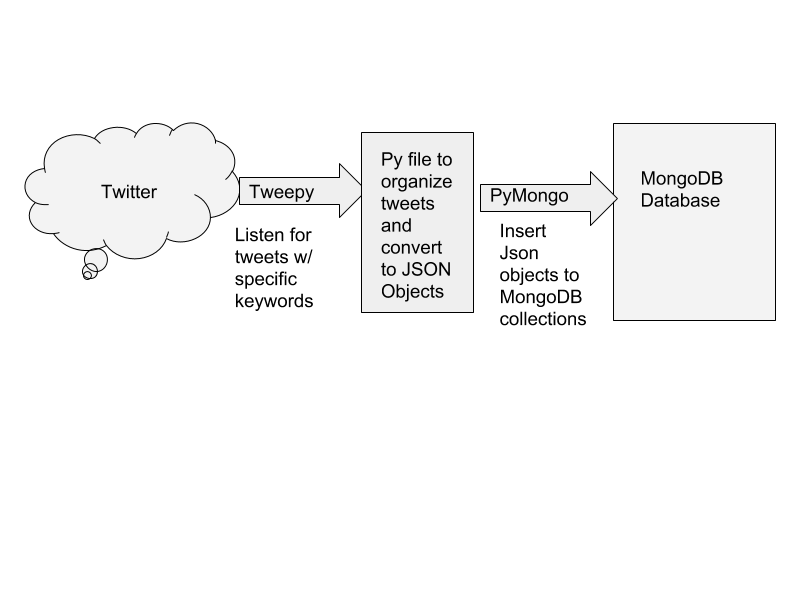
\includegraphics[scale=0.5]{data_collection}
\end{figure}
\begin{enumerate}
	\item Building a tweet streamer to "listen" to tweets based on keywords
	\item Preprocessing the tweets
	\item Storing processed tweets in a database. 
\end{enumerate}
The pipeline was built in python3. The code for it can be found in Appendix A


\section{Streaming Tweets}
\hspace{0.1in} There are two ways to gather tweets using Tweepy (the Python Twitter API). The first is to query a profile or a search term. This method is not preferred for several reasons. First, Twitter has put a hard cap on the number of tweets each query can return at one time. This means that querying will be in-exact and time consuming loop. Next, Twitter's search function will naturally promote tweets that have more engagement. This means that tweets with more likes and retweets, comments, and followers will get preference, which results in a biased data set. 

The other way to gather tweets is to stream tweets. A Tweepy stream monitors live twitter content and returns all tweets that contain a given set of keywords. Streaming has the disadvantage of gathering only live tweets - it does not search tweets from before it started running. But, streaming has the advantage of gathering any tweets that meet the keyword requirement, irrelevant of engagement. 

The code written to stream tweets can be found in Appendix A. The streamer is a abstracted in the Twitter API. To use it, the user must fill in several methods. The methods defined here are on\_connect, on\_error, and on\_data. The first two are trivial. On\_connect is used to connect, and confirms once the stream is live. If the stream crashes - which can happen because of several reasons - on\_error will return exactly which error caused the stream to malfunction. 

The last method on\_data is where the tweets are received and processed. Each tweet is received as a dictionary. The keys are attributes of the tweet (i.e. date and time, text, user, etc.). From there any processing is up to the user; the tweet's text can be printed, the tweets can be prepared for entry to a data base, etc. More on that later. 

\section{Databases}
\hspace{0.1in} Before describing how the database for this project works, it's important to have a basic grasp of databases. A database is a structure that stores data, usually in the form of documents or objects. 

%Re-Write After significant research
%Re-write entire section - do definitions go in the appendix? Ask Stefan
\subsection{MongoDB and NoSQL}
\hspace{0.1in} For years most databases had been operated and queried using SQL or Structured Query Language. This language worked off the idea that documents were stored in tables. It's organization made it incredibly efficient. A drawback of the efficiency was that queries to the databases ended up being unnecessarily complicated. 

NoSQL databases - as inferred from the name.- databases that aren't operated using SQL. They also lack the table structure of SQL databases. MongoDB is an open-source database that stores objects as JSONS. It looks something like this;

\begin{figure}[h]
	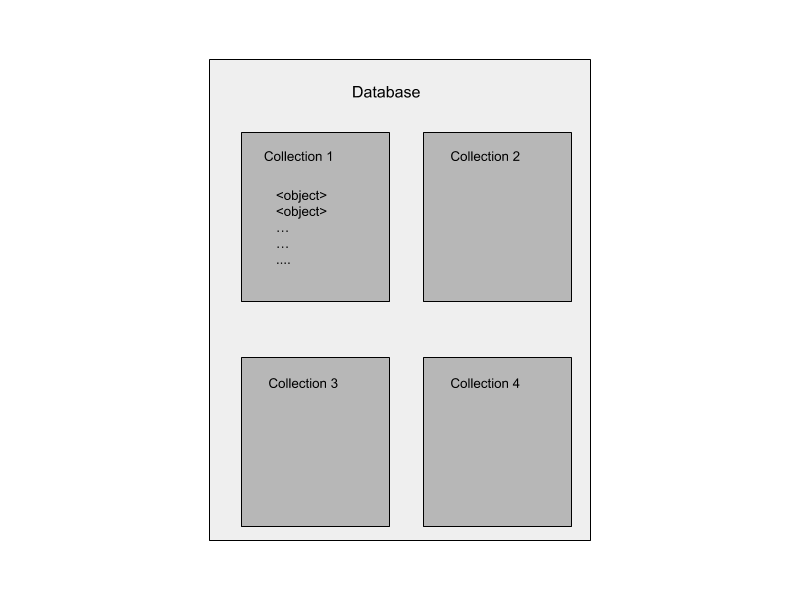
\includegraphics[scale=0.5]{database}
\end{figure}

Each database will contain a variety of collections. These collections are where the objects themselves are actually stored. Having multiple collection allows the user to organize their database. Each object also has a series of attributes. These attributes work like a tagging system and are used as search terms. 

\section{Adding Tweets to a MongoDB}
\hspace{0.1in}The code written in Appendix A shows the actions for adding the streamed tweets to a MongoDB database. It uses commands provided by the Python MongoDB API known as PyMongo. 

All mongo actions take place in the on\_data method. First, the mongo client is initialized. The client is what interacts with the database. The tweet which is stored as a dictionary is converted to json using the json python package. Then, tweet is added to a collection in the database.

\begin{appendices}
\chapter{Data Collection Code}

The following code is used to gather tweets for various elections. To change which election is being monitored, the keywords need to be changed. To change the storage destination, change the past for the variable MONGO\_HOST.

\lstinputlisting[language=Python]{misc_listener.py}

\end{appendices}


\bibliographystyle{plain}
\bibliography{midwaybib}
\end{document}